\documentclass{article}
\usepackage{graphicx,subfiles,amsmath,amsfonts,bookmark,float}
\usepackage{hyperref}
\usepackage[left=2cm, right=2cm, top=2cm, bottom=2cm]{geometry}

\hypersetup{
    colorlinks=true,
    linkcolor=blue,
    filecolor=magenta,      
    urlcolor=cyan,
    pdftitle={Overleaf Example},
    pdfpagemode=FullScreen,
    }

\title{Workshop 0: Intro to GT PACE}
\author{Supercomputing@GT}
\date{}

\begin{document}

\maketitle

\tableofcontents

\section{What is PACE?}

\textbf{PACE} stands for the \textbf{Partnership for an Advanced Computing Environment}. PACE provides leading-edge high-performance computing resources for Georgia Tech faculty, students, and staff that require them. PACE offers:

\begin{itemize}
    \item CPU/GPU Compute Capacity
    \item Individual \& Shared Project Storage
    \item Classroom \& Teaching Resources 
    \item Various software support 
    \item User Support \& No-Cost Consultation Sessions 
    \item Monthly Trainings, Workshops, \& Other Learning Events 
    \item User Documentation \& Video Recordings 
\end{itemize}

\noindent PACE maintains 5 different compute clusters. They are respectively called:

\begin{itemize}
    \item \textbf{Phoenix}: Research cluster open to GT/GTRI faculty. 
    \item \textbf{ICE}: Educational cluster for courses teaching HPC concepts. 
    \item \textbf{Firebird}: Research cluster for Controlled Unclassified Information, International Traffic in Arms Regulations (ITAR), and export controlled data.
    \item \textbf{Buzzard}: High throughput pool connected to OSG's OSPool; designed for researchers with many small independent jobs
    \item \textbf{Hive}: Research cluster only available to recipients of the NSF MRI award \#1828187 and their collaborators.
\end{itemize}

\noindent As you can see, it is likely that most of you will interact mostly with the ICE cluster throughout your GT career. However, the skills we teach in this workshop will carry over to the other clusters since all PACE clusters use the same underlying job scheduling technology, Slurm. 

\subsection{References}

For more information on PACE, please visit the following pages:
\begin{itemize}
    \item \url{https://pace.gatech.edu/participation/}
    \item \url{https://gatech.service-now.com/technology?id=kb_article_view&sysparm_article=KB0042503}
\end{itemize}

\section{Getting Started with PACE}

\subsection{Accessing the PACE Cluster}

\subsubsection{Preliminary: Make sure that you are connected to the GT VPN!}

If you don't know what I mean about the ``GT VPN'', install the GlobalProtect VPN Client using OIT's directions:
\begin{itemize}
    \item Windows: \url{https://gatech.service-now.com/home?id=kb_article_view&sysparm_article=KB0026742}
    \item MacOS: \url{https://gatech.service-now.com/home?id=kb_article_view&sysparm_article=KB0026743}
    \item Ubuntu: \url{https://gatech.service-now.com/home?id=kb_article_view&sysparm_article=KB0028027}
\end{itemize}

Once the VPN is downloaded, you can move on to the next section.

\subsubsection{SSH Instructions}

\textbf{SSH}, or the Secure Shell Protocol, is a cryptographic network protocol for operating network services securely over an unsecured network. In most cases, it will be the way you access remote computers in your future programming career. Read more about ssh here: \url{https://en.wikipedia.org/wiki/Secure_Shell}. Use the following steps to connect to a PACE-ICE login node.

\begin{enumerate}
    \item Connect to host: \texttt{ssh <gt-username>@login-ice.pace.gatech.edu}
    \item Type in your GT password upon seeing the prompt. \textbf{Note.} Nothing will show up as you type.
    \item If you've successfully logged in, you'll see a prompt like the following:
    \begin{figure}[H]
        \centering
        
\includegraphics[width=0.5\textwidth]{img/Screenshot 2025-09-07 at 22.55.10.png}
    \end{figure}
    You are now in a login node of the cluster, which you will use to access files on the cluster, write code, and submit jobs. 
\end{enumerate}

\subsubsection{Remote SSH w/ VSCode}

For those who are using VSCode, there's a handy extension from the VSCode extension store that you can use in order to use VSCode in your remote environment. The extension is called \textbf{Remote - SSH} by Microsoft itself: \url{https://marketplace.visualstudio.com/items?itemName=ms-vscode-remote.remote-ssh}. 

\subsection{Obtaining Interactive Compute Nodes}

You are now ready to interact with the PACE-ICE compute nodes! You can obtain interactive compute resources using the \texttt{salloc} command. The following command is an example of how you may allocate an interactive computer node:

\begin{center}
    \textcolor{red}{\texttt{salloc -N1 --ntasks-per-node=4 -t1:00:00}}
\end{center}

\noindent Hmm, what does this all mean? The stuff thats written after \texttt{salloc} are the arguments that are passed into the \texttt{salloc} command to tell it how to behave. The arguments' meanings are given below:

\begin{itemize}
    \item \texttt{N1}: Allocate 1 node.
    \item \texttt{--ntasks-per-node=4}: 4 tasks can run in parallel on each node.
    \item \texttt{-t1:00:00}: This job should run for 1 hour. 
\end{itemize}

\noindent  The previous command essentially told the cluster to give us access to 1 node (which would have a CPU), and allow 4 tasks to be run in parallel on that node. The cluster should also give us access to this compute resource for exactly an hour. Once we run the command, a job request will be submitted and we will be added to the job request queue like good citizens. \\ 

\noindent You can also get GPUs by passing different flags!

\begin{itemize}
    \item \texttt{--gres=gpu:<gpu type>:<number of gpus per node>}: Specifies the number of GPUs per node.
    \item \texttt{--gpus=<gpu type>:<total number of gpus>}: Specifies the number of GPUs per job. 
\end{itemize}

\noindent For example, let us get an NVIDIA H200 in interactive mode!

\begin{center}
    \texttt{salloc -N1 --ntasks-per-node=2 --gres=gpu:H200:1 -t1:00:00}
\end{center}

\subsection{Aside: A Brief Overview of Linux Bash}

So far, you may be uncomfortable with the fact that there does not appear to be a graphical user interface (GUI) for you to interact with PACE. Unfortunately, for must supercomputing cluster environments in the world, no GUIs will be provided, even for login nodes. In most cases, users must interact with the environment just by typing shell commands into the \texttt{ssh} terminal. This may seem intimidating at first, but don't be scared! We will start you off with some basic commands that are most common which you may need throughout this workshop and future basic workflows. \\ 

\noindent \textbf{Note.} The following conventions are used in the list of commands below:
\begin{itemize}
    \item \textbf{Directory}: Contains a list of files. This is equivalent to folders on Mac and Windows OS. 
    \item \textbf{File Tree}: This is the hierarchical structure that Linux uses to organize its files and directories, starting from the root directory \texttt{/}. 
    \item \textbf{Filepath}: This is the position of a file or directory relative to where you are located in the file tree. 
    \item \texttt{<...>}: This notation indicates an argument that may or may not be passed to the command. 
    \item \texttt{[...]}: This notation indicates a part of the command that is not strictly necessary, i.e., an optional argument. 
\end{itemize}

\noindent This is the list of some of the most common Bash commands that you will find most useful when you begin working with Linux shells. 

\begin{itemize}
    \item \texttt{pwd}: Print the current directory's name. 
    \item \texttt{cd <directory-name>}: Change directory.
    \item \texttt{ls [<directory-name>]}: List directory.
    \item \texttt{mkdir <directory-name>}: Make directory. 
    \item \texttt{touch <file-name>}: Create file.
    \item \texttt{cat <filepath>}: View contents of file without opening it. 
\end{itemize}

\noindent While our workshop will not focus much on working in the Bash terminal, it will be important for you to at least be familiar with Bash in order to work with supercomputer clusters in the future as we explained above. To learn more about Bash, a starting point is here:

\begin{itemize}
    \item \url{https://www.w3schools.com/bash/index.php}
\end{itemize}

\noindent It should also be noted that there are actually a lot of shell programs out there which may have their own quirks and differences from Bash. Bash is just a shell program that a system admin chose to use over other shell programs. In fact, in many cases you can actually switch to using different shells depending on your preference! Some other kinds of shell programs that you may have seen includes:

\begin{itemize}
    \item \texttt{Z shell} (\url{https://en.wikipedia.org/wiki/Z_shell}) -- especially for Mac users; and
    \item \texttt{C shell} (\url{https://en.wikipedia.org/wiki/C_shell}) -- for those who may have used Red Hat Linux.
\end{itemize}

\subsection{Hands-On Practice}

We now allocate some time for you to be able to get familiar with using PACE! For this workshop, we have prepared an optimal implementation of matrix multiplication using \textbf{MPI}, which is a library that is commonly used for HPC programming by following the message-passing paradigm. You will run this program using a compute node on PACE to familiarize yourself with the PACE environment as well as check out the true power of supercomputing!

\begin{enumerate}
    \item As taught in section 2.1, \texttt{ssh} into the PACE instruction cluster using either a simple terminal software or VSCode (or any other IDE of your choice).
    \item Download the programs onto your login node with the command: \\ \textcolor{red}{\texttt{git clone https://github.com/suco-gt/}}
    \item Compile the code following the instructions in the repository's README. 
    \item Allocate an interactive node with 16 cores for 30 minutes!
\end{enumerate}

\noindent \textbf{Note.} You will NOT need to allocate a GPU for this workshop. If you want to work with a GPU come to our NVIDIA CUDA workshop!

\section{A Brief Intro to Slurm and Slurm Jobs}

Up till now, you've actually already been working with Slurm to obtain interactive compute nodes! However, you may notice that there is a problem. Your computer needs to be kept open to ensure that you remain connected to the compute node, because your interactive job will terminate as soon as your session is disconnected. This does not seem very practical if we are trying to train a very large neural network model or perform multi-day climate simulations. This is where \textbf{Slurm Jobs} come to the rescue. 

\subsection{But what is Slurm?}

The \textbf{Slurm Workload Manager} is a free and open-source job scheduler for Linux and Unix-like kernels. Today it is the workload manager used by about 60\% of the TOP500 supercomputers. Originally it was developed in a collaborative effort by the Lawrence Livermore National Lab, SchedMD, Linux NetworX, Hewlett-Packard, and Groupe Bull. Nowadays it is mainly maintained by SchedMD. \\

\noindent So what is a \textbf{job scheduler}? A job scheduler is software for controlling unattended background program execution of jobs. This allows for long-running programs to be left running unattended until finished, or allow automated execution of short-running programs. \\ 

\noindent As a job scheduler, Slurm offers three main features:

\begin{itemize}
    \item Allocation of compute resources for variable duration with different kinds of access levels. 
    \item Assurance of fairness and arbitrating contention for limited resources by managing a queue of pending jobs.
    \item Provide a framework for starting, executing, and monitoring background work.   
\end{itemize}

\noindent In summary, Slurm is the backbone of many of today's large computing clusters, including GT's PACE. Without Slurm, the world will descend into chaos and misery as programmers battle each other for exclusive access to the latest GPUs and CPUs. 

\subsection{How to use Slurm Jobs}

So how do we create a Slurm job that can be submitted to a supercomputing cluster? The process is extremely simple. Rather than passing in numerous parameters and manually allocating computer resource with the \texttt{salloc} command we previously used, we create a \textbf{batch script} instead, and submit the script to the cluster using the \texttt{sbatch} command on the login node. We can then use other useful Slurm comamnds such as \texttt{squeue} to interact with and learn about our submitted jobs. \\

\noindent The batch script that we write is similar to the shell scripts that we would write. These Slurm batch scripts can always be broken down into two sections: the arguments section and the commands section. An example of the batch script is given below, followed by an explanation of what each section is. 

\begin{figure}[H]
    \centering
    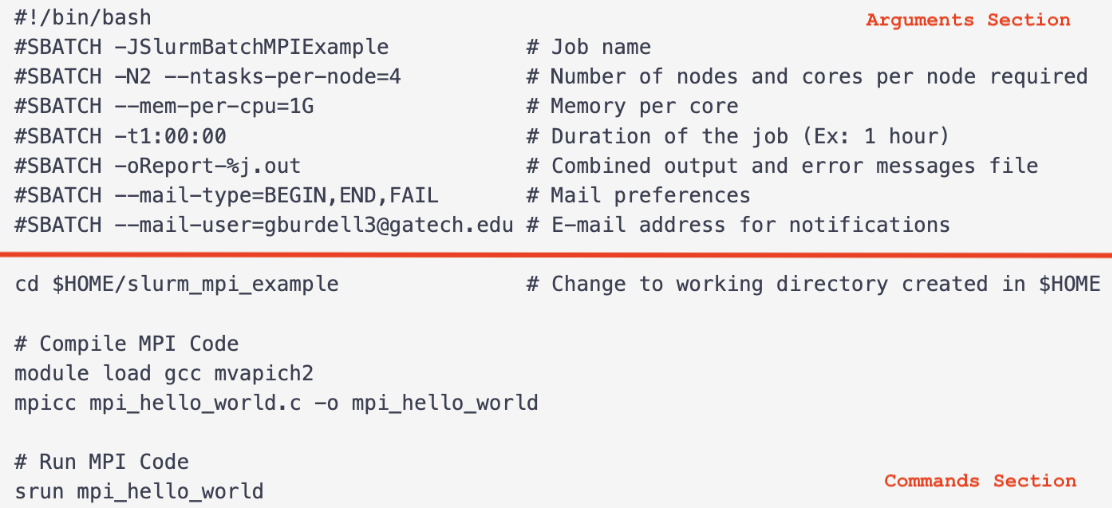
\includegraphics[width=0.9\textwidth]{img/Screenshot 2025-09-07 at 21.59.40.png}
    \caption{An example batch script.}
\end{figure}

\noindent The arguments section is where we tell Slurm the environment in which our job should be run. We do so by passing in the arguments we previously used in the \texttt{salloc} command by instead writing them on separate lines at the start of the batch script, with each argument being marked by a \texttt{\#SBATCH} at the start of the line, followed by the argument we want to pass. \\ 

\noindent After the arguments section comes the commands section, where we tell the compute resource that Slurm eventually allocates for our job the commands that should be run. You can generally just use the same commands that you needed to use in order to run your program on an interactive compute node.

\subsection{Hands-On Practice}

We ran out of time in the workshop to allow for some practice submitting Slurm jobs. However, we believe that you now have all the knowledge that is necessary for you to learn how to submit a Slurm job for running the programs that we have given you today! If you are a participant, you will have 1 more week's access to ICE-PACE, so make sure to take this opportunity to practice your newly obtained skills!

\subsection{References}

For more information on the usage of Slurm on PACE, Slurm itself, and job scheduling in general, you can visit the following pages:

\begin{itemize}
    \item \url{https://docs.pace.gatech.edu/training/img/Phoenix%20Slurm%20Orientation%20v5.pdf}
    \item \url{https://gatech.service-now.com/technology?id=kb_article_view&sysparm_article=KB0042503}
    \item \url{https://slurm.schedmd.com/documentation.html}
    \item \url{https://en.wikipedia.org/wiki/Job_scheduler}
    \item \url{https://en.wikipedia.org/wiki/Distributed_computing}
\end{itemize}

\end{document}
